\slide{Conclusão}{

    Realizou-se a predição de fluxo de veículos em vias urbanas a curto prazo (15, 30, 45, 60 minutos no futuro), para isso:

    \begin{itemize}
        \item Implementou-se a análise e transformação dos dados adquiridos;
        \item Implementou-se os modelos de aprendizagem de máquina escolhidos;
        \item Realizou-se uma busca pelos melhores valores de parâmetros e hiper-parâmetros;
        \item Treinou-se os modelos com os dados processados;
        \item Automatizou-se a comparação dos modelos;
    \end{itemize}
}

\slide{Análise dos Resultados}{
    \begin{itemize}
        \item Modelos tradicionais foram capazes de aprender de maneira mais precisa a distribuição do conjunto de dados utilizado;
        \item Todos os modelos propostos se saíram melhor do que as bases de comparação;
        \item Os modelos treinados com o conjunto de dados A, que possui menos atributos, tiveram uma tendência a obter melhores predições;
    \end{itemize}
    
}


\slide{Contribuições}{

    \begin{itemize}
       \item  Proposta de uma métrica de avaliação que não é comumente utilizada em problemas de predição de fluxo de veículos (\(\alpha\));
       \item Caracterização do conjunto de dados;
       \item Validação dos modelos para cenários com cruzamentos;
    \end{itemize}
}

\slide{Trabalhos Futuros}{
    \begin{itemize}
        \item Treinar os modelos com pelo 1 ano de dados;
        \item Polir a representação da coluna Data para os modelos;
        \item Utilizar múltiplos sensores para predição;
        \item Utilizar modelos paramétricos;
        \item Incluir modelos não paramétricos mais complexos;
        \item Aprofundar a escolha de hiper-parâmetros;
    \end{itemize}
}

\slide{Considerações Finais}{
    Os integrantes dessa apresentação agradecem aos professores que os ajudaram ao longo do desenvolvimento do trabalho, visto que no início dos estudos, os mesmos não possuíam familiaridade com o tema, nem com as linguagens e bibliotecas necessárias para a realização dos experimentos. Portanto, pode-se dizer que o aprendizado pessoal de cada um com a realização do trabalho foi de grande valia.
}

\slide{Dados e Código}{
    \begin{itemize}
        \item Código utilizado se encontra em:  \url{https://github.com/claudiosegala/Monografia/tree/master/code}
        \item Dados utilizados se encontram em: \url{http://bit.ly/processed-data-2l5MaAG}
    \end{itemize}
}

% \slide{Códigos}{
%     \begin{figure}[]
%         \centering
%         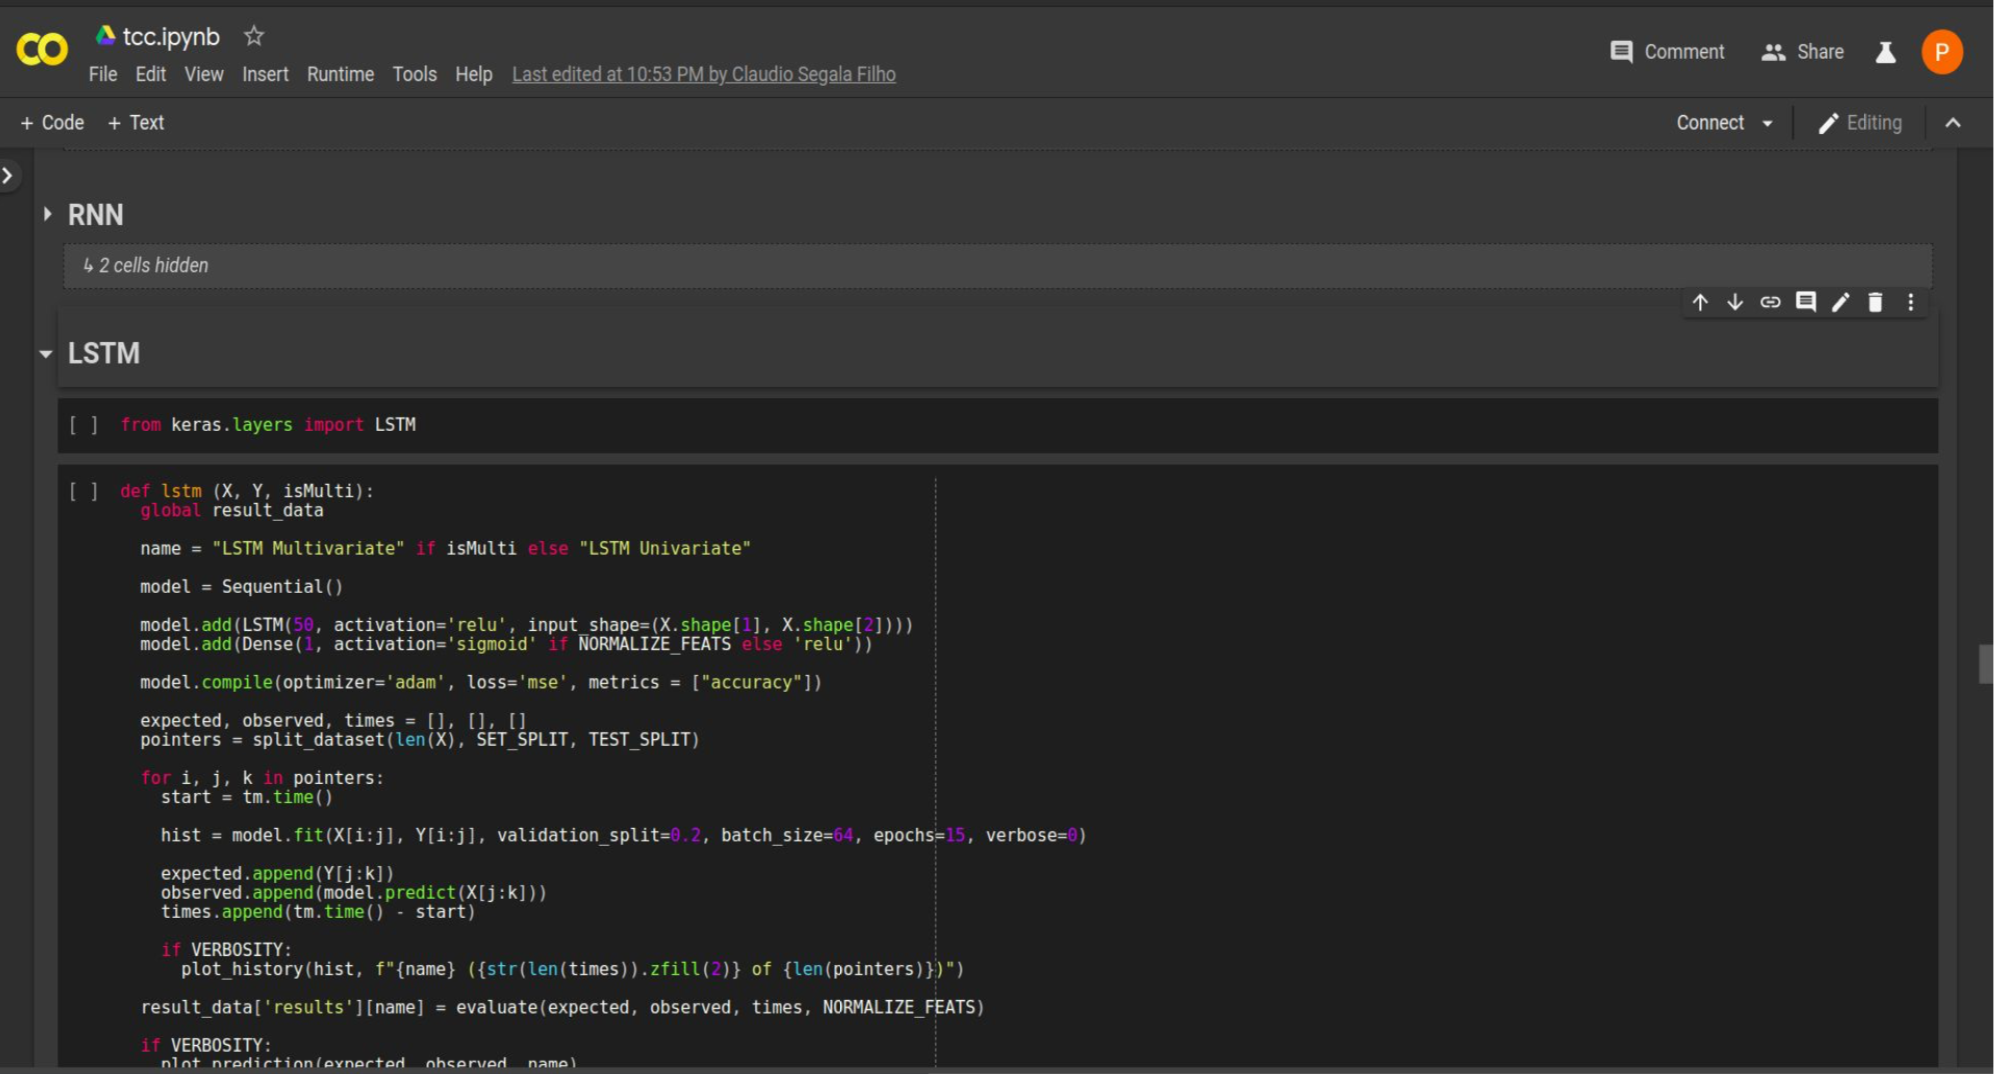
\includegraphics[scale=0.25]{img/colab.png}
%         \caption{Código utilizado disponível na plataforma Google Colab}
%         \label{fig:colab}
%     \end{figure}
% }

% \slide{Dados}{
%     \begin{figure}[]
%         \centering
%         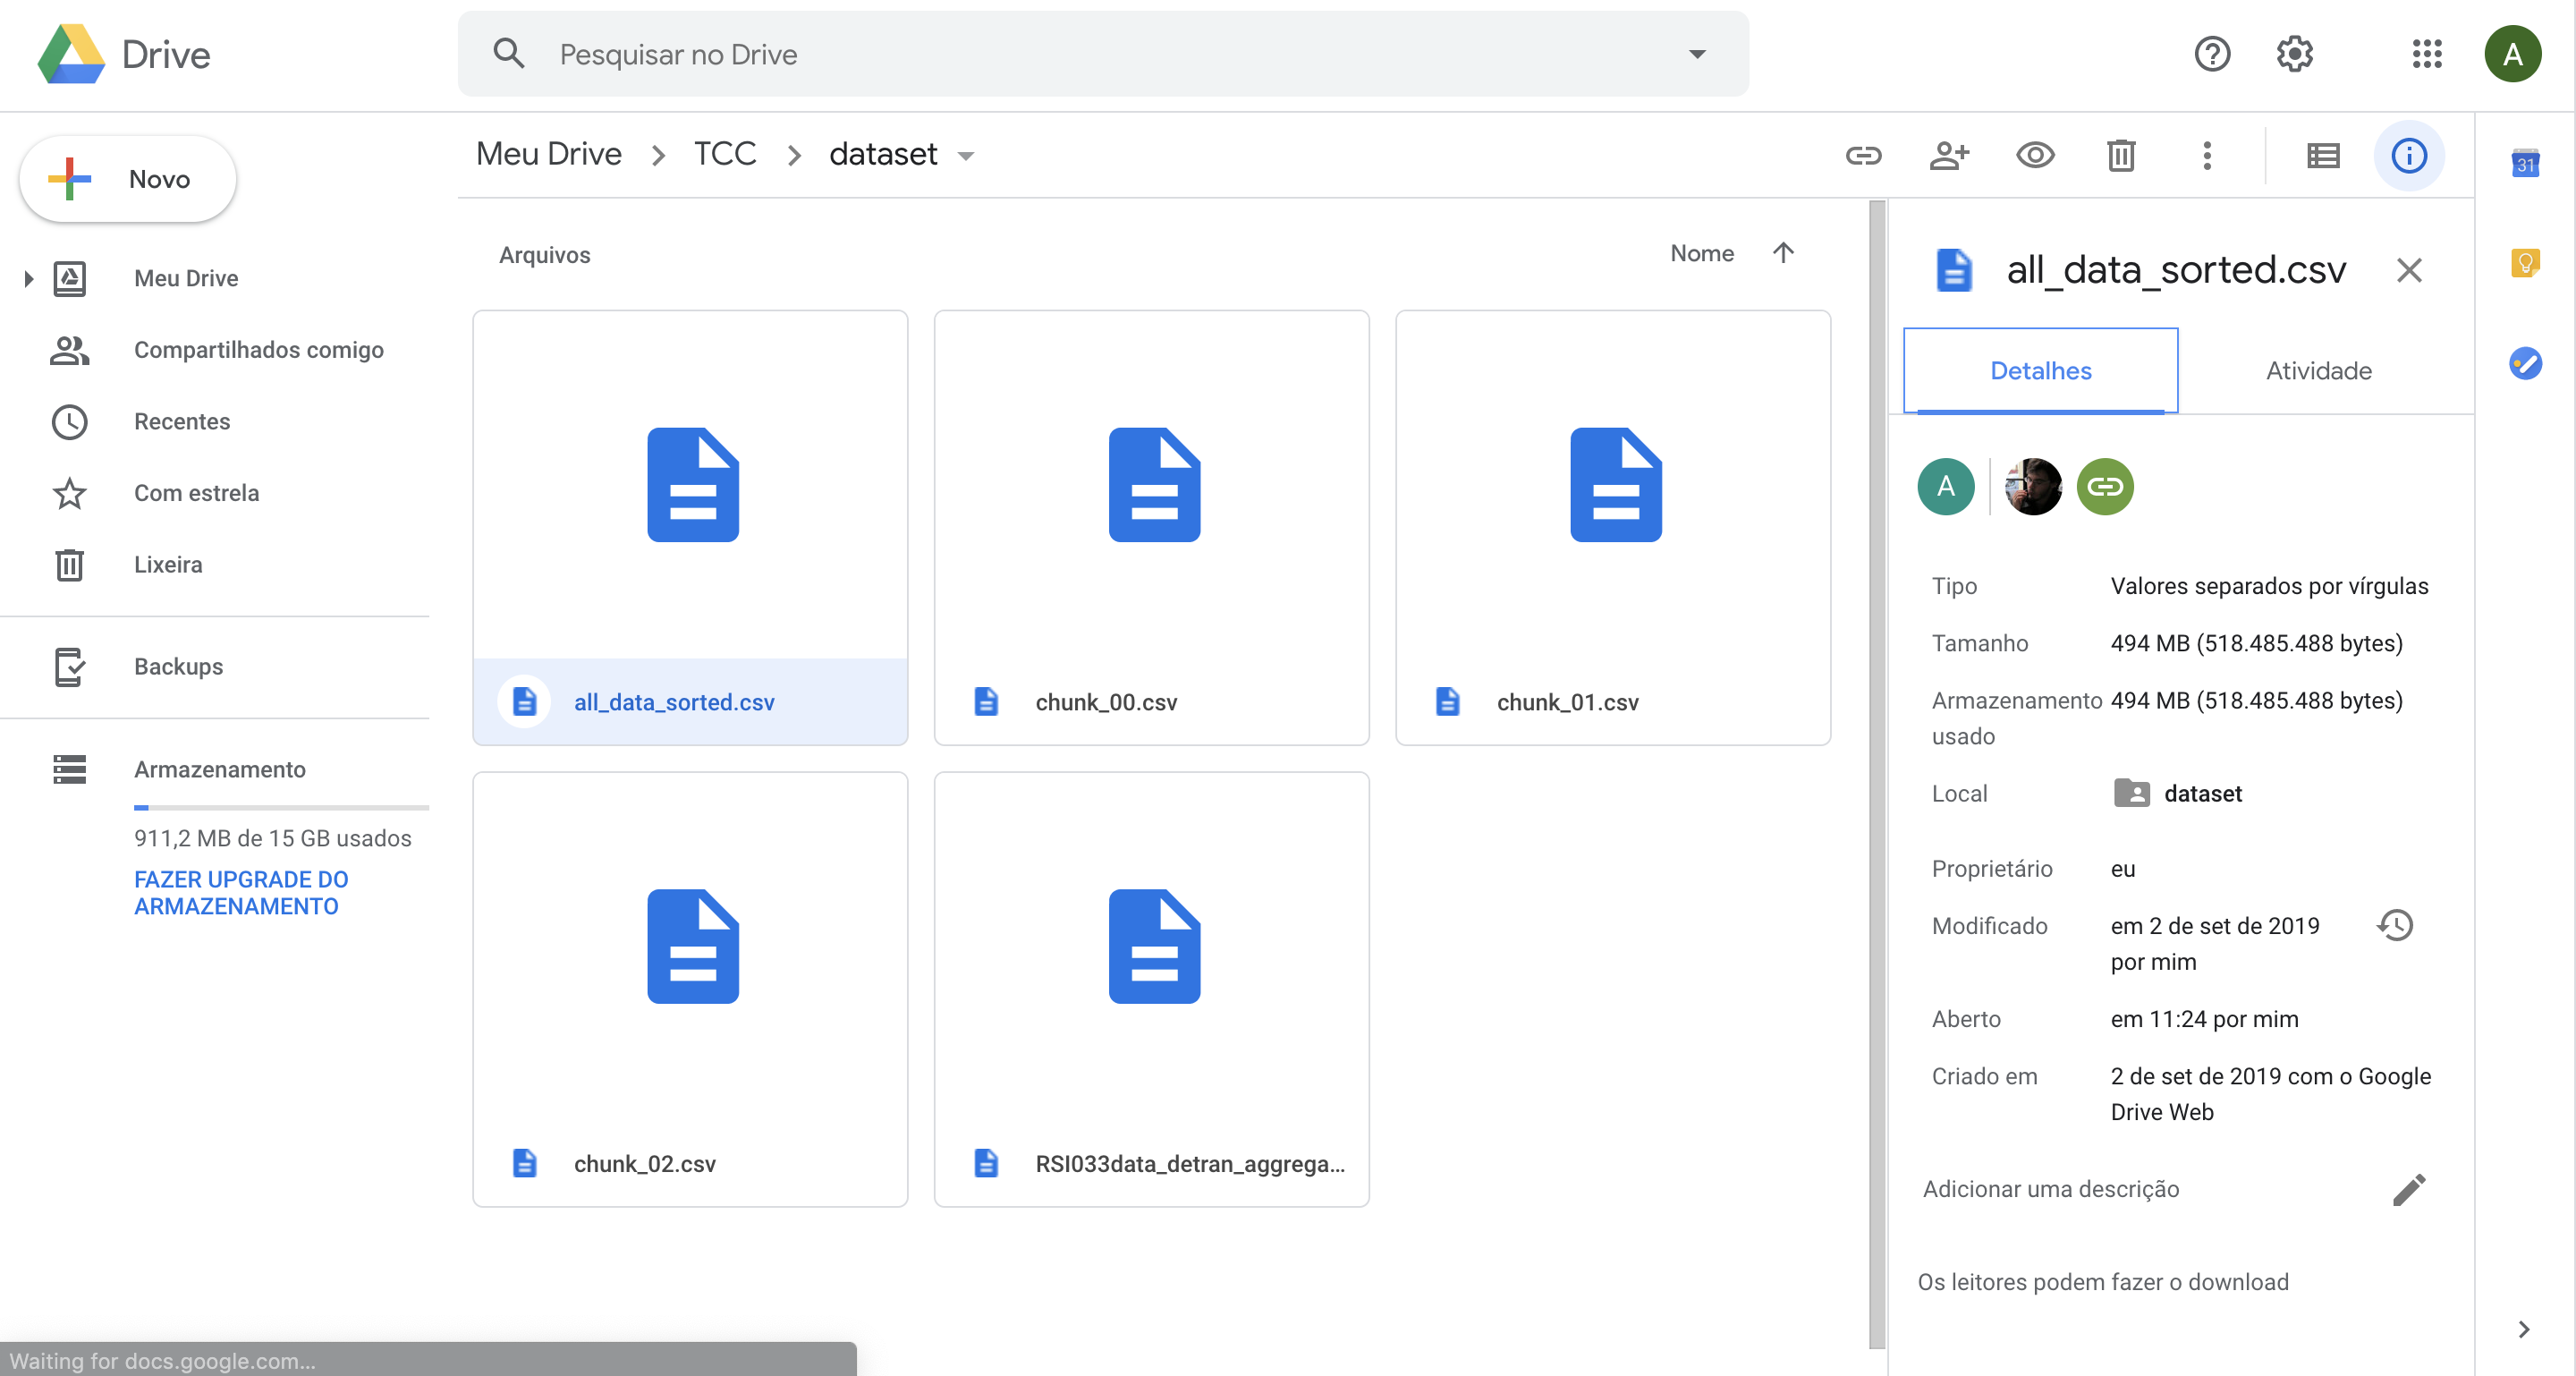
\includegraphics[scale=0.25]{img/dataset_drive.png}
%         \caption{Dados utilizado disponível na plataforma Google Drive}
%         \label{fig:dataset_drive}
%     \end{figure}
% }